\documentclass{article}
\usepackage{tikz}
\usetikzlibrary{positioning}

\begin{document}

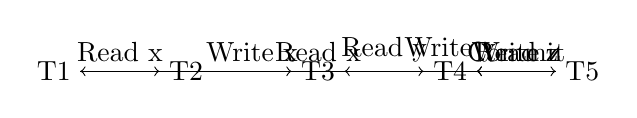
\begin{tikzpicture}[node distance=1cm]
    \node (T1) {T1};
    \node[right=of T1] (T2) {T2};
    \node[right=of T2] (T3) {T3};
    \node[right=of T3] (T4) {T4};
    \node[right=of T4] (T5) {T5};

    \draw[->] (T1) -- node[above] {Read x} (T2);
    \draw[->] (T2) -- node[above] {Write x} (T3);
    \draw[->] (T3) -- node[above] {Read y} (T4);
    \draw[->] (T4) -- node[above] {Write z} (T5);

    \draw[->] (T5) -- node[above] {Read x} (T1);
    \draw[->] (T5) -- node[above] {Write y} (T3);
    \draw[->] (T5) -- node[above] {Read z} (T4);
    \draw[->] (T5) -- node[above] {Commit} (T4);
\end{tikzpicture}

\end{document}